% !TeX root = ../thuthesis-example.tex

\chapter{利用重要性采样对训练过程加速}\label{chapter5}
\section{引言}
这个章节主要讲了将重要性采用的方法应用于\ref{chapter4}中设计的模型的训练过程的加速。
参考相关的工作,搭建了一个,基于最新版本的深度学习框架的,
对于各类神经网络通用的训练加速的框架,介绍了框架的具体实现的方式,及其加速的效果。

\section{训练加速算法}
需要指出的是,不同的样本在不同的研究阶段对模型的训练效果是不一样的。
基于训练加速这一研究目标,这里从样本的角度出发,研究如何尽可能高效地利用样本,
在每个训练阶段选择对当前训练最有效果的样本来进行训练。
那么需要定义怎样算对训练有效果,以及怎么选择合适的选择样本的策略。

\begin{algorithm}
  \caption{重要性采样算法}
  \begin{algorithmic}
    \STATE 输入:$B$、$b$、$\tau_{th}$
    \STATE $t \gets 1$
    \STATE $\tau \gets 0$
    \REPEAT
      \IF {$\tau > \tau_{th} $}
        \STATE $P \gets$从标准分布中采样$B$个点
        \STATE 计算$P$中所有点的分数$S$
        \STATE 重采样:$Q \gets$从这$B$个点中抽取$b$个点
        \STATE 权重:$w_i \gets \frac{1}{B*S_i}$,$\forall i \in P$
        \STATE $\theta_t \gets $sgd\_step($w_i$,$Q$,$\theta_{t-1}$)
      \ELSE
        \STATE $Q \gets$从标准分布中采样$b$个点
        \STATE 权重:$w_1 \gets 1$,$\forall i \in Q$
        \STATE $\theta_t \gets $sgd\_step($w_i$,$Q$,$\theta_{t-1}$)
      \ENDIF
      \STATE update $\tau$
    \UNTIL{convergence} 
  \end{algorithmic}
\end{algorithm}

\section{基于重要性采样的训练加速方法框架的设计}
本文中提到的训练加速框架是基于新版本Tensorflow 2.4的基础上完成,
应用了最新的Tensorflow的Keras接口。
新版本Tensorflow中集成了Tensorflow的灵活性,和Keras接口的高度抽象简单易用的特点。
以往的框架往往是基于旧版本的Tensorflow或Keras编写而成,
对于新版本的模型没办法调用框架来进行加速。
相对于以往的框架而言,
本系统结合了动态图和静态图的优点,模块逻辑清晰而且运行效率高。

而且框架适用于各类神经网络,对具体神经网络的结构没有限制和要求。

\subsection{模型结构设计}

\begin{figure}
  \centering
  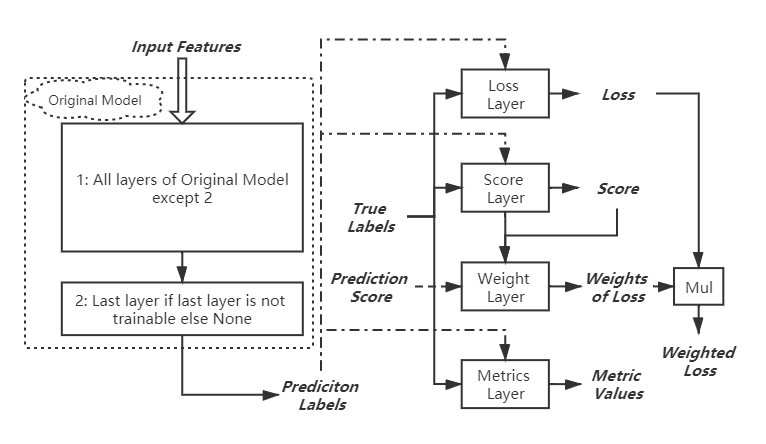
\includegraphics[width=1.1\linewidth]{figures/重要性采样模型结构.png}
  \caption{重要性采样模型结构}
  \label{fig:importance-sampling-model}
\end{figure}

如图\ref{fig:importance-sampling-model}画出了应用重要性采样的模型构建。
整体模型架构是在原有的模型的基础上搭建完成的,在原来的模型的层后面又加入了额外的层,
这些层用到了原来模型的输出作为输入,同时引入了一些其他的数据如标签数据作为输入,
得到额外的输出。

主要的附加层是这四种,下面对它们进行分别的介绍。
\begin{enumerate}
  \item Loss layer:得到的样本的损失函数值。
  \item Score layer:得到的结果用来衡量样本的重要性,
  用于筛选样本,及决定样本的梯度下降的权重。
  有几种可以选择的类型:
  "loss"、"gnorm"、
  "full\_gnorm"、"acc"
  \item Weight layer:会根据每个样本的分数计算得到样本的损失的权重。
  \item Metrics Layer:计算得到评价指标。
\end{enumerate}

\section{训练加速实验效果}

  在下面的实验中,应用前面提到的重要性采样的方法,对模型进行加速,并和原始模型的结果进行对比。
  为了消除随机性的影响,同时验证方法的鲁棒性,每组实验进行三次,会给出平均的结果,和三组分别的结果,进行比对。
  为了保证公平,同一次实验中,对比的两种训练方式会加载同样的模型初始化参数。

  \subsubsection{加速效果}
  \begin{figure}
    \centering
    \begin{subfigure}[b]{0.45\textwidth}
      \centering
      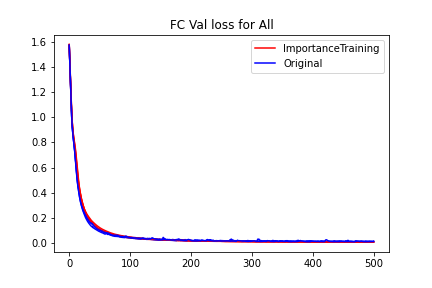
\includegraphics[width=\textwidth]{20210326_2324/FC Val loss for All.png}
      \caption{FC}
      \label{fig:FC Val loss for All}
    \end{subfigure}
    \hfill
    \begin{subfigure}[b]{0.45\textwidth}
        \centering
        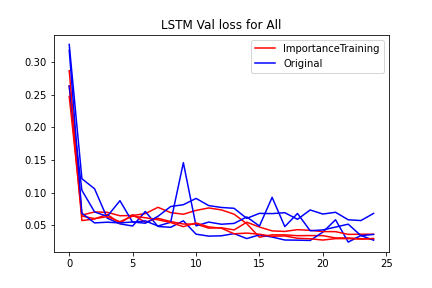
\includegraphics[width=\textwidth]{20210326_2324/LSTM Val loss for All.png}
        \caption{LSTM}
        \label{fig:LSTM Val loss for All}
    \end{subfigure}
    \caption{三次对比实验训练加速平均效果:验证集的loss变化趋势图}
    \label{fig:importance-sampling-performance}
  \end{figure}

  \begin{table}
    \centering
    \caption{重要性采样的效果:数据随机划分下,全连接网络测试集上的MSE结果}
    \begin{tabular}{lclclcl}
      \toprule
      结果类型       & 重要性采样方法 & 对比实验 & MSE比例(<1为有效果)                                     \\
      \midrule
      三次实验平均   & 0.053 & 0.069 & 0.759 \\
      实验1    & 0.055 & 0.084 & 0.651                                \\
      实验2 & 0.054 & 0.057 & 0.948                                     \\
      实验3 & 0.049 & 0.067 & 0.733                  \\
      \bottomrule
    \end{tabular}
    \label{tab:fc random test mses}
  \end{table}

  \begin{table}
    \centering
    \caption{重要性采样的效果:数据随机划分下,长短时记忆网络测试集上的MSE结果}
    \begin{tabular}{lclclcl}
      \toprule
      结果类型       & 重要性采样方法 & 对比实验 & MSE比例(<1为有效果)                                       \\
      \midrule
      三次实验平均   & 0.096 &  0.147 & 0.652 \\
      实验1    & 0.097 &  0.142 & 0.681 \\
      实验2 & 0.109 & 0.124 & 0.882                                     \\
      实验3 & 0.082 & 0.175 & 0.467                  \\
      \bottomrule
    \end{tabular}
    \label{tab:lstm random test mses}
  \end{table}

  图\ref{fig:importance-sampling-performance}中给出了,应用不同模型,
  在应用和不应用重要性采样的方法下,多次实验,验证集loss的变化平均趋势对比,
  直接这样看看不出加速效果。

  从\ref{fig:FC Val loss for All}和\ref{fig:LSTM Val loss for All}中加速前后的对比,
  我们可以看出,应用方法的初期,采样其实比较接近标准的采样方式,
  其实不会有太大的加速效果。

  但是从\ref{tab:fc random test mses}和\ref{tab:lstm random test mses}中的结果来看,
  训练同样的epochs,明显应用了重要性采样方法进行训练加速的最终结果要好很多,最终的MSE的值的比例
  在加速后:加速前=0.6\textasciitilde 0.8左右。
  加速效果比较明显。

  \begin{figure}
    \begin{subfigure}[b]{0.45\textwidth}
        \centering
        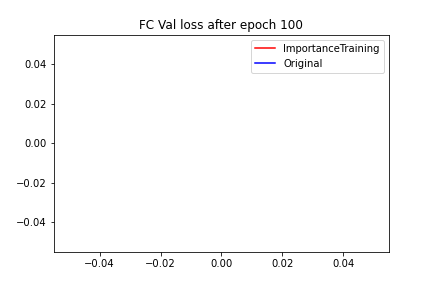
\includegraphics[width=\textwidth]{20210326_2324/FC Val loss after epoch 100.png}
        \caption{FC (after 100 epochs)}
        \label{fig:FC Val loss after epoch 100}
    \end{subfigure}
    \hfill
    \begin{subfigure}[b]{0.45\textwidth}
        \centering
        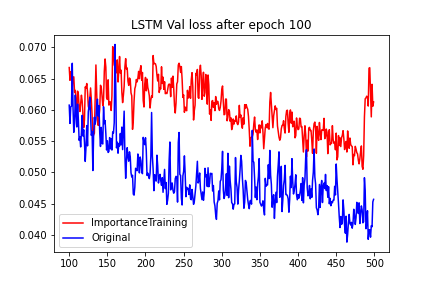
\includegraphics[width=\textwidth]{20210326_2324/LSTM Val loss after epoch 100.png}
        \caption{LSTM (after 100 epochs)}
        \label{fig:LSTM Val loss after epoch 100}
    \end{subfigure}
      \caption{三次对比实验训练加速平均效果:验证集的loss变化趋势图(100个epoch开始)}
      \label{fig:importance-sampling-performance-after-100}
  \end{figure}

  \subsubsection{加速效果的稳定性}
  \begin{figure}
    \centering
    \begin{subfigure}[b]{0.45\textwidth}
        \centering
        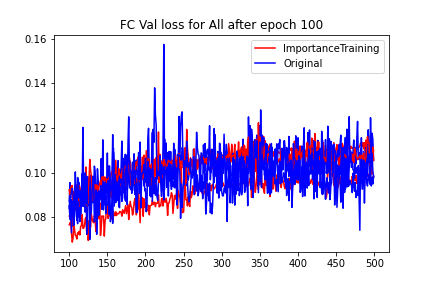
\includegraphics[width=\textwidth]{20210326_2324/FC Val loss for All after epoch 100.png}
        \caption{FC (after 100 epochs)}
        \label{fig:FC Val loss for All after epoch 100}
    \end{subfigure}
    \hfill
    \begin{subfigure}[b]{0.45\textwidth}
        \centering
        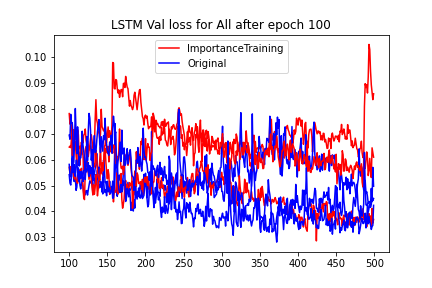
\includegraphics[width=\textwidth]{20210326_2324/LSTM Val loss for All after epoch 100.png}
        \caption{LSTM (after 100 epochs)}
        \label{fig:LSTM Val loss for All after epoch 100}
    \end{subfigure}
      \caption{三次对比实验分别的训练加速效果:验证集的loss变化趋势图}
      \label{fig:importance-sampling-performance-All}
  \end{figure}

  需要注意的是,由于前100个epoch的对比不是很明显,
  \ref{fig:importance-sampling-performance-after-100}中的
  图\ref{fig:FC Val loss after epoch 100}和
  图\ref{fig:LSTM Val loss after epoch 100}
  对100个epoch以后的数据单独plot了出来。
  明显应用了重要性采样加速的验证集loss下降更快。

  本文中应用的重要性采样的方法会有比较稳定的加速效果,
  如图\ref{fig:importance-sampling-performance-All}中所示,
  重要性采样方法处理后的模型,
  相比原来的模型,应用不同的模型分别进行的三次实验中,loss下降的速度都要更快。
  多次实验结果比较一致,反映了加速效果会比较稳定,
  说明整个加速框架比较鲁棒,不太会受到随机因素的影响。

\section{本章小结}
本章主要介绍了应用重要性采样方法对模型进行训练加速的相关内容。
从实验的结果可以看出,整体的加速效果较好,而且加速效果比较稳定,
说明加速系统比较鲁棒。

